\chapter{Introduction}
\label{chap:1}
\ChapterPageStuff{1}

\section{Background}\label{section:background}

Software maintenance according to the \textit{IEEE Standard 1219}\footnote{\textbf{IEEE Standards} documents are developed within the Technical Committees of the IEEE Societies, and the Standards Coordinating Committees of the IEEE Standards Board \cite{Mamone1994}.} is the process that includes the following phases \cite{Mamone1994, Hasan2012}:
\begin{itemize}
	\item Identifying the problem or modification and classification of it
	\item Analysis of the identification of the maintenance issue
	\item Design of the solution to implement maintenance
	\item Implementation of the solution
	\item System testing of the modified software system
	\item Acceptance test on the fully integrated system
	\item Delivery requirements met of the modified software system
\end{itemize}

%TODO Beter definisie vir technical debt
The maintenance problems or modification are regularly identified and usually addressed based on an initial priority ranking. This priority ranking is determined by using classification models to determine which type of maintenance needs to be done (adaptive, corrective, perfective and preventive) \cite{Tang2010,Mamone1994,Ping2010}.\par Continuous analysis of the identified maintenance problems or modifications enables the software engineers and developers to create a preliminary plan to address these issues \cite{Port2017}. Technical debt can exist in almost every software system and should be correctly managed by analysing which maintenance issues should be prioritised \cite{DeLeon-Sigg2020, Reimanis2016}.\par Implementing a suitable maintenance framework to resolve the identified issues reduces the technical debt. Various maintenance models can be used to solve these issues when implementing any one of the maintenance types. Identifying and analysing these are issues is the most challenging part of software maintenance \cite{DeLeon-Sigg2020}.

\subsection{Maintenance in software systems}
Most companies will strive to increase their digital products and services over the software project's life cycle to maximise their profits \cite{Gralha2018}. This will increase the maintenance that needs to be done on both new and old systems \cite{Niu2018, Galster2019, Hasan2012}. Although maintenance is essential for software systems, most companies do not have a defined maintenance model or process to guide them when implementing maintenance \cite{Stojanov2017}. Software maintenance is an essential task in software development, and it can directly reduce cost and effort to create new software systems or modify it \cite{FrancisThamburaj2017}.\par A study about software maintenance was conducted by the United States Department of Commerce. They found that the total development cost can be as much as $60\%$-$80\%$ of the total cost for the software system's development life cycle \cite{Ogheneovo2014, Stark1996, Ackermann2009,Tang2010}. These costs will increase (as shown in \Cref{fig:CH1_Costs_of_fixing_bugs}) to maintain much older and more complex software systems, therefore implementing maintenance can keep the software system feasible in its entire life cycle \cite{Alenezi2016, Booch1986}.

\begin{figure}[!htb] % An h :here, t: top, b: bottom.
	\centering % cent the figure
	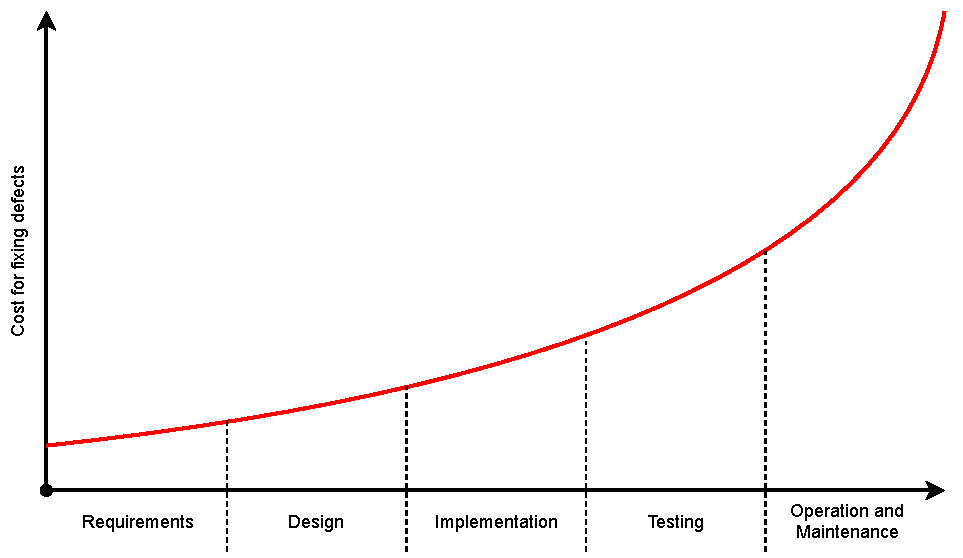
\includegraphics[width=0.5\textwidth]{Chapter1/Cost_of_fixing_bugs/Cost_of_fixing_bugs.pdf}
	\caption[Cost of fixing software system defects]
	{\textit{Cost of fixing software system defects \cite{Ogheneovo2014}}}\label{fig:CH1_Costs_of_fixing_bugs}
\end{figure} 

Maintenance of software systems is continuous and is a reduced form of software development and is aimed to modify software systems while preserving its integrity \cite{Sneed2004,Ackermann2009,Port2017}. In \Cref{tbl:CH1_MaintenanceTypes}, adaptive and perfective maintenance types are most effective when maintaining a software system's integrity. Most software engineers and developers will implement these two significant types of maintenance in their maintenance procedures.\par Adaptive and perfective maintenance ensures the software system will continue to evolve to meet the system requirements to ensure that it is useable and feasible. This is also the most effective way of reducing technical debt by adapting the software system. This continuous improvement uses about $70\%$ of the maintenance resources to manage the maintenance of the software system \cite{Kumar2013}. 

\begin{table}[!htb]
	\centering
	\small
	\caption[Software maintenance types]
	{\textit{Software maintenance types \cite{Ping2010,Hasan2012,Mamone1994}}}
	\label{tbl:CH1_MaintenanceTypes}
	\begin{tabularx}{\textwidth}{|c|X|c|}
		\hline
		\textbf{Maintenance type} & \textbf{Description} & \textbf{$\%$ of maintenance activities} \\ \hline
		Adaptive & \raggedright Adaptive maintenance in software systems is any modification or enhancements to keep it usable with a changing or changed software environment. & $\approx 35.5\%$ \\ \hline
		Perfective & Perfective maintenance based are modifications made based on the change of the end-user's new requirements. It can also improve the performance or maintainability of the software system in its life cycle. & $\approx 35.5\%$ \\ \hline
		Corrective & \raggedright Corrective maintenance are improvements made to fix certain defects or errors in a software system. & $\approx 20\%$ \\ \hline
		Preventive & \raggedright  Preventive maintenance are improvements made to software systems that prevents problems in the future. & $\approx 5\%$ \\ \hline
	\end{tabularx}
\end{table}

It can be demanding task to prioritise the available resources to certain parts of the software system to do maintenance to prevent or fix any software defects \cite{Mamone1994, Hasan2012}. The defect density can measure the software's quality in \Cref{eq:Defect_Density} for specific time period \cite{Shah2012, Alenezi2016}. The defect density of a software system is the is number of possible defects divided by the size of the software system.  A lower defect density indicates an improved version of the software system.

\begin{equation}
	\label{eq:Defect_Density}
	Defect~Density = \frac{CNDD}{KLoC},
\end{equation}

where:

\begin{itemize}
	\item $CNDD$ is the cumulative number of defects in the post release version of the software system
	\item $KLoC$ (thousands lines of code) is the size of the observed executable code in a software system 
\end{itemize}

In open source software systems the defect density increases due the number of developers working on the same software system and the size of the system itself \cite{Rahmani2010}. Adding more developers to improve a software system may not always have positive improvement in each of the maintenance types in \Cref{tbl:CH1_MaintenanceTypes}. There might be even a need to increase the corrective maintenance efforts as more developers are already trying resolve the existing maintenance issues.\par The size of the software system in OSS does have an impact on the defective density \cite{Rahmani2010}. Naturally larger and more complex software system will have larger defect density as the system will be complex and some parts of it will be older than others \cite{SourceForged2009}. 

In \Cref{fig:CH1_Costs_of_fixing_bugs}, the cost of maintenance increase if the maintenance activities increase when implementing the four major types of software maintenance. These maintenance activities cannot be neglected as the software will most likely keep evolving as new features are added to keep it useable \cite{Alenezi2016}. \par In an ideal situation, the maintenance should be done with the software development planning phase. Due to time constraints and available resources, it is not easy to plan any maintenance phase for most software engineers and programmers. The cost increases of maintenance due to lack of planning or preventive measurements to keep the quality software from degrading \cite{Alenezi2016}.

\subsection{Problems with implementing software maintenance}\label{sec:Maintenance_problems}

Under most circumstances, maintenance is implemented if a software system does not meet the required functions specified by the performance requirements \cite{Ogheneovo2014, Sneed2004}. These systems will also most likely have multiple software defects or will be extremely complex due to:

\begin{itemize}
	\item \textbf{Problem domain being complex:} The software may not be well defined or structured. This is due to how large the software systems grow over their entire life cycle or duplicate software components that are made. This is caused by poor understanding of the system architecture by developers not doing the required maintenance on these systems and just adding new features \cite{Galster2019, Booch1986}.
	\item \textbf{Difficulties of managing development process:} Most companies will strive to increase their digital products and services over the life cycle of the software project to maximise possible profits with the resources invested \cite{Niu2018}. Increasing production of the development process will only strain to maintain software systems \cite{Sneed2004}.\par The development team needs to prioritise concrete tasks in the development process to make the project feasible by just focusing on these tasks can lead to poor decisions are made about the required task to perform software maintenance \cite{Galster2019, Ogheneovo2014, Lenarduzzi2017}. 
	\item \textbf{Flexibility of the software:} Trying to predict what the possible future architecture may look like and modifying it while preserving the software's integrity may be difficult in software maintenance \cite{Garlan1999}. Software is flexible if it is adaptable to the problem domain when adding modifications to it \cite{Ogheneovo2014}.\par Most development teams will follow a software development methodology to create a future architecture that is modular and structured to preserve the development integrity of new software \cite{Vijayasarathy2016, Rehman2018}. This will also have an impact on the type of maintenance activity (as in \Cref{tbl:CH1_MaintenanceTypes}) the development team will use, which are called corrective, perfective, adaptive and preventive maintenance \cite{FrancisThamburaj2017, Hasan2012, Stojanov2017, Snipes2018}.
	\item \textbf{Change in user's requirements:} In software development, the users will often request new additional requirements to the software systems delivered to them \cite{Ogheneovo2014}. Modifying software systems may include new additional features that change the initial system architecture. Maintenance of these systems is crucial to ensure that existing components of the system will work as intended with the new components that are added.
\end{itemize}

\subsection{Software maintenance model}
%TDOD Example maybe not relevant
A software maintenance model is an abstract representation of software systems' evolution to keep track of all the maintenance activities when implementing software maintenance \cite{Ren2011}. The \textit{IEEE Standard 1219} for software maintenance is the standard that should be followed when planning the software maintenance as in \Cref{fig:CH1_IEEE_Model}.\par It is crucial to identify the maintenance that should be done before making, which will start with the user or developer's request to modify the software. A feasibility analysis of any changes that are required is made. A certain amount of resources will be needed to implement maintenance, and this will impact the design and implementation phase. System and acceptance testing are essential to ensure that the system is still fully functional. After the system is thoroughly tested and approved, it will be available to the user, and the maintenance process will start again when there are new improvements made for the software system.

\begin{figure}[!htb] % An h :here, t: top, b: bottom.
	\centering % cent the figure
	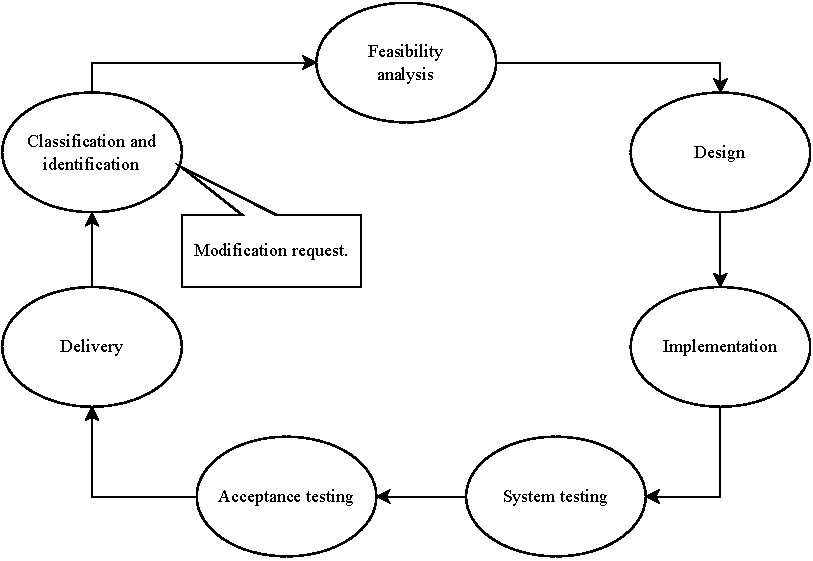
\includegraphics[width=0.6\textwidth]{Chapter1/IEEE_Model/IEEE_Model.pdf}
	\caption[IEEE model]
	{\textit{IEEE model \cite{Ren2011}}} \label{fig:CH1_IEEE_Model}
\end{figure}

Most organisations maintenance model will be based on \Cref{fig:CH1_IEEE_Model} to manage their maintenance efforts. About $50\%$ of the developer implementing maintenance job is to understand what the software system is supposed to do, and the changes they make will not change the intended functionality of the system \cite{Tang2010, Zhuo}. This is due to the problems with implementing maintenance as discussed in \Cref{sec:Maintenance_problems}.\par \Cref{fig:CH1_MaintenanceFlow} example of what a practical maintenance flow model an organisation would likely use to implement software maintenance. Initially, a developer will complete a request form or issue indicating a new problem or feature request that needs to be implemented \cite{Tang2010}.\par If the issue is a problem in the software system, the severity of the problem needs to assess to decide on the priority level to resolve it. This type of maintenance is mostly corrective and can also be preventive if it is a possible solution to prevent any software failures in the future \cite{Tang2010}. Other types of maintenance requests are either adaptive or perfective and usually placed in the development team's task queue.\par After all the maintenance tasks are defined, the development team will prioritise the higher-rated issues that need to be solved. This process will repeat itself until all the task in the for that specific software system is completed.\par To fully follow the \textit{IEEE Standard 1219} of implementing maintenance on a software system, the defects or areas of improvements are identified. Utilisation analysis of event logs can be used to detect any hidden defects or performance issues in a software system to implement software maintenance \cite{Cinque2013, Rong2018a, Levin2019}.

\begin{figure}[!htb] % An h :here, t: top, b: bottom.
	\centering % cent the figure
	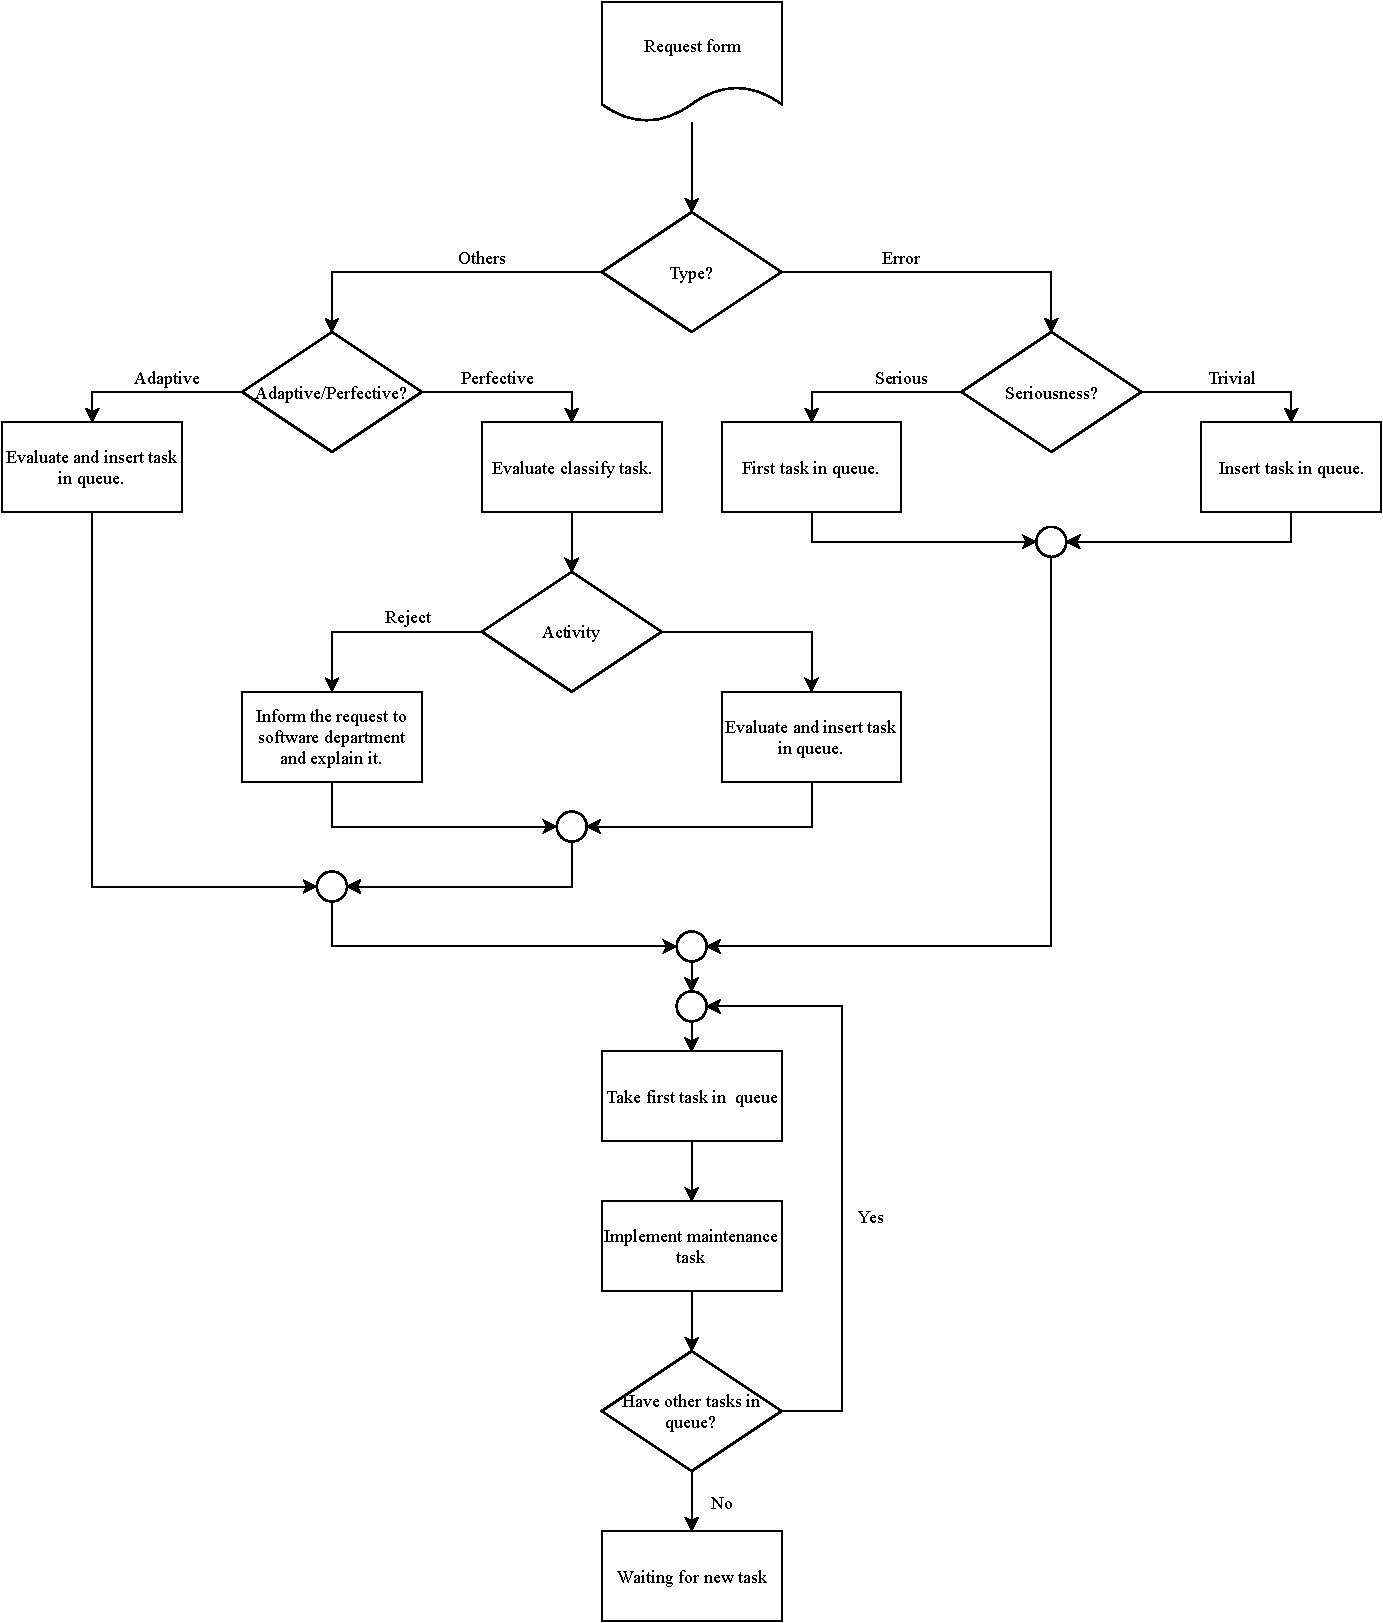
\includegraphics[width=0.85\textwidth]{Chapter1/Maintenance_flow/Maintenance_Flow.pdf}
	\caption[Maintenance flow model]
	{\textit{Maintenance flow model \cite{Tang2010}}} \label{fig:CH1_MaintenanceFlow}
\end{figure}

%TODO hier is waar need of study moet begin 
%TODO What is the problems with What is the problem with event logging
%TODO How can analysis improve maintenance
\clearpage

\section{Event logging}\label{sec:EventLogging}

An event log $W$ is the sequence of log entries of events $E$ or a multi-set of traces when $T$ is a finite set of defined tasks being done and $T^+$ is a set of all the non-empty finite sequences of $T$ \cite{Kherbouche2017}

\begin{equation}
	\label{eq:LogEvent}
	W = (E, C, A, \partial, \wp, \Gamma, \succ) \subseteq T^+,
\end{equation}

where:

\begin{itemize}
	\item $E$ is a finite set of events,
	\item $C$ is a finite set of cases,
	\item $A$ is the finite set of additional data that can be split up into disjoint sets of event attributes (timestamps $T_S$, cost $O$, resources $R$, event types, $E_T$ and data elements $D$),
	\item $\partial$ is the \textit{surjective}\footnote{\label{ftn:Surjective}A \textbf{surjective} function is a way of matching the members of a set $A$ to a set $B$ \cite{Szendrei1990}.} $E\rightarrow C$,
	\item $\wp$ is the \textit{surjective}\footref{ftn:Surjective} $A\rightarrow E$,
	\item $\Gamma$ is the \textit{surjective}\footref{ftn:Surjective} $E\rightarrow T$,
	\item $\succ \subseteq E\times E$ is the total ordered events in $E$ that belongs to a specific case that is called a trace.
\end{itemize}

As mentioned in \Cref{section:background}, software maintenance can make use of event logs to improve software maintenance. It is a common practice in the software industry to record any detailed system run-time information into logs to be analysed later by developers or software engineers to solve software related problems with the system as in \Cref{tbl:CH1_EventLogsUsage} \cite{Zhu2019}.

\begin{table}[!htb]
	\centering
	\small
	\caption[Event logs usage]
	{\textit{Event logs usage}}
	\label{tbl:CH1_EventLogsUsage}
	\begin{tabularx}{\textwidth}{|l|X|}
		\hline \textbf{Usage} & \textbf{Description} \\
		\hline Debugging of software systems & Able to diagnose software failures for both testing and production environments \cite{Rong2018a}.\\
		\hline Anomaly detection & Event logs can be used to detect any abnormal system behaviour using an anomalous detection algorithm using logging data \cite{Gurumdimma2016}. This can also be used to find any vulnerabilities in the software environment \cite{Dwyer2013}. \\
		\hline Performance diagnosis & Software performance is important to producing quality software \cite{EvangelinGeetha2007,Baccanico2014}. These is mostly performance logs of software systems that are used to monitor the software system, which is useful for resource tuning, load balancing and checking system scalability \cite{Song2017}. \\ 
		\hline Error and failure analysis & Event logs are used to analyse the failure behaviours of software systems which enables engineers to understand the failure modes of the system, find the root cause of these failures, prevent them and improve the reliability of the future releases of the system \cite{Cinque2013}.\\
		\hline Analysis of security alerts & In any software environment or information technology infrastructure, security is a major concern for any organisation \cite{Pathan2014, Dwyer2013}. It is important to know the overall security status of the software system \\
		\hline
	\end{tabularx}
\end{table}

The technique to collect numeric or textual data that describes the behaviour of a computer system is called event logging \cite{Pecchia2015, Baccanico2014}. Event logs are collected textual data containing the records of events that happened in a software system and is used for system management tasks as in \Cref{tbl:CH1_EventLogsUsage} \cite{Rong2018a, Rong2018, Baccanico2014}.

%TODO \chapter{Logging practice in software engineering}

\subsection{Logging quality}\label{sec:CH1_LoggingQuality}

Software engineers and developers will need to make informed logging decisions to cover the necessary run-time information without negatively impacting the software system's performance \cite{Zhu2015,Zhu2019,Kherbouche2017}. This does not ensure that there may be some problems using logging in software systems, and the most common issues with event logging is:

\subsubsection{Quantity of the logs:} 
%TODO Reword to not use "bad"
It can become difficult to log every event in a software system as these systems will get larger and more complex during their development life cycle \cite{Stojanov2017}. It would be bad too not log enough information during run-time as the necessary information about the event will make the postmortem analysis of the software system incomplete. However, it is not always the best solution to log every possible event \cite{Zhu2015, Jans2012}.

\subsubsection{Quality of event logs} 
The logs' quantity is necessary, but there may be unnecessary extra logs that will only take storage space that is not useful for log analysis. The logs' accuracy and consistency are critical when making reliable decisions based on the identified behaviour of the software system with the historical data that exists in the logs \cite{Stojanov2017,Kherbouche2017}.\par An event log quality model is essential to ensure that the logs will be of high-quality for the data mining process in \Cref{sec:SystemUtilisation}. The data in an event log should be accurate, available and complete to ensure that the correct decisions can be made from the log analysis \cite{Kherbouche2017, VanDerAalst2011}.

\begin{figure}[!htb] % An h :here, t: top, b: bottom.
	\centering % cent the figure
	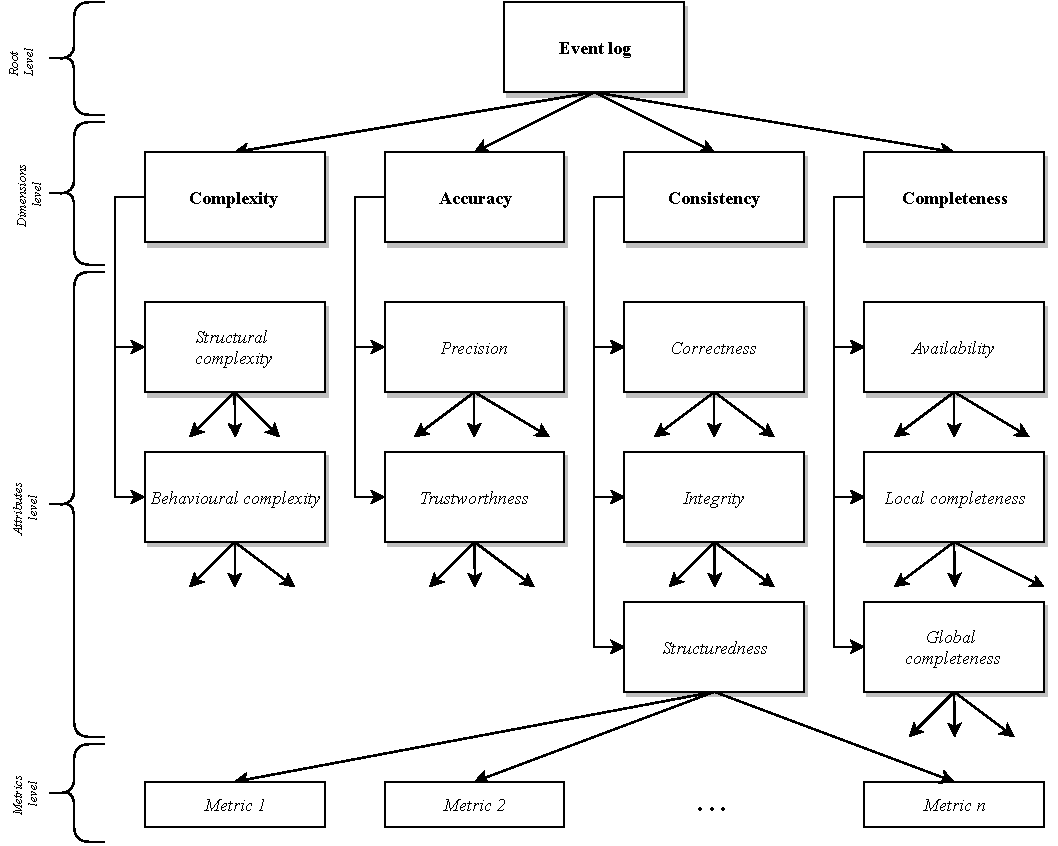
\includegraphics[width=0.9\textwidth]{Chapter1/Event_Log_Model/Event_Log_Model.pdf}
	\caption[The event log quality model]
	{\textit{The event log quality model \cite{Kherbouche2017}}} \label{fig:EventQModel}
\end{figure}

\subsubsection{Performance cost of logging} 
%TODO Also data storage costs
Creating logging mechanisms will need additional code to be written in the software system to obtain the event logs. Software logging will consume additional system resources like the processor and storage of the host computer system. It is unacceptable to have noticeable performance issues due to the logging on the rest of the system operations. Therefore the logging mechanism needs to be efficient to get the necessary details about the event that took place \cite{Zhu2015,Zhu2019}. 

\clearpage

\subsection{Logging parsing and log points}\label{sec:Ch1_LoggignPoints}
Knowing what to log can significantly reduce any overhead the logging mechanism may produce in the software system \cite{Jia2018, Pecchia2015}. Preserving quality (as described in \Cref{sec:CH1_LoggingQuality}) is a necessity to ensure that the logs that are obtained will fulfil its purpose when doing analysis on it.\par Before the logs can be parsed to structured dataset the key attributes needs to be defined that will describe the event log \cite{Bekeneva2020a}. The attributes in describe in \Cref{tbl:CH1_Log_Basic_Attributes} are the most basic attributes a log event should have. They make it possible to mine and analyse the logs based on their attributes and increases the precision and reliability of the event log \cite{Kherbouche2017}.

\begin{table}[!htb]
	\centering
	\small
	\caption[Basic log event attributes]
	{\textit{Basic log event attributes \cite{Bekeneva2020a}}}
	\label{tbl:CH1_Log_Basic_Attributes}
	\begin{tabularx}{\textwidth}{|c|X|}
		\hline \textbf{Attribute} & \textbf{Description} \\
		\hline Case number & Unique identifiers for each individual log event. This is usually the primary identifier for the log event. \\
		\hline Timestamp & The time and date that the log event occurred. This is part of identifying the order of events or trace along with the case number of the event log \cite{Kherbouche2017}. \\
		\hline Event type & Each log event can be grouped with other log events that have similar actions that happened. These event type attribute needs to be classified based on a state change, failure to execute a instruction, or due to an occurrence of an activity like the availability of a service \cite{Fedaghi2010}. \\
		\hline Resource & These sources which the event took place at. This can be parts of the software that performs the event action or was the caused for the event to be initiated by another part of the software. \\
		\hline Other meta data & This any other relevant information that can be used as the event log's attribute that further expand the information of the log event. This can be one extra field or many other individual attribute fields.\\
		\hline
	\end{tabularx}
\end{table}

The case number and timestamp attributes in \Cref{tbl:CH1_Log_Basic_Attributes} can be defined anytime during the logging process. This is not the cas for the rest of the attributes. Every log should have a defined action that will put it in a group of logs that can be defined as event type. These event types can be either predefined of what is expected from the event action or will need to be observed later analysis of the logs in case there is no clear grouping of the logs \cite{Bekeneva2020a, Fedaghi2010}.\par The sources of the log event assist on determine the location where the event took place. For event logs this essential to try recreate scenario or action based on the relevant parts of the software system participated in the event action.\par Other meta data can increase the log quality by providing additional information about software instructions that were executed. These attributes adds more information that can be used to recreate the scenario or action that may be unique parameters or other events that participated in the event log.\par To get the attributes in \Cref{tbl:CH1_Log_Basic_Attributes} a instruction generates the log and parse it on to a data set. These log instructions are called logging points in software environment \cite{Pecchia2015, Zhu2015}. They can be any instruction such as print function that displays the information for the user to more complex functions or libraries that can be created by third party developers.

\clearpage

In \Cref{fig:Log_Parsing} is an example of a logging point parsing a log message in a structured log. The defined attributes are captured by the logging point when the event take place or occurred. The created log message is then parsed into a structured lof to be safe in database or displayed. The logging point should strategically placed to captured the nesseacary attributes to complete the log event \cite{Fedaghi2010}.

\begin{figure}[!htb] % An h :here, t: top, b: bottom.
	\centering % cent the figure
	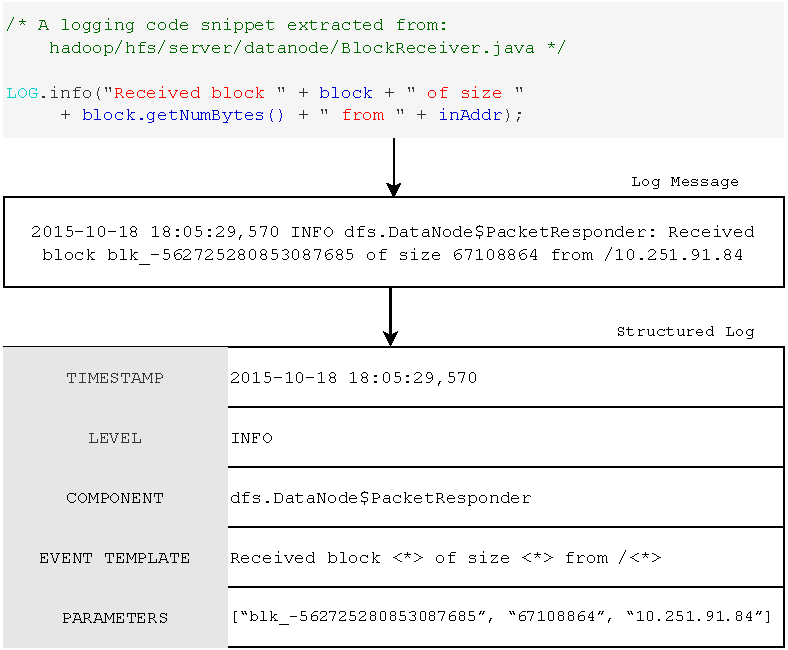
\includegraphics[width=0.7\textwidth]{Chapter1/Log_Parsing_Example/Log_Parsing_Example.pdf}
	\caption[An illustrative example of log parsing]
	{\textit{An illustrative example of log parsing \cite{Zhu2019}}} \label{fig:Log_Parsing}
\end{figure}

Determine where to place the logging point in a giving software is directly impacted by what the attributes are and if the captured log will be of high quality as described in \Cref{sec:CH1_LoggingQuality}. The availability of consistent high quality logs will directly impact the process mining in the analysis of the logs \cite{Kherbouche2017}.\par To strategically place a logging point developers needs to consider what the activation of the logging point will be during the runtime of the software system \cite{Pecchia2015,Cinque2013}. The activations can be simple if statement that meets a certain criteria or instructions that execute after when an event or action took place (e.g. runtime errors).

\clearpage

\section{System utilisation analysis}\label{sec:SystemUtilisation}

\clearpage

\section{Objectives of the study}
This study aims to develop a logging mechanism to track user-based activities to perform analysis of these logs to improve system maintenance in a software environment. The study is divided into two components to achieve the primary goal, which is the design and implementation of the logging mechanism and the analysis of the system utilisation to improve system maintenance.

\subsection{Logging mechanism:}
\begin{itemize}
	\item Random text.
\end{itemize}

\subsection{Analysis of the system utilisation to improve software maintenance}
\begin{itemize}
	\item Random text.
\end{itemize}

\section{Overview of the dissertation}
\subsubsection{Chapter 1: Introduction}
This chapter contains the background of software maintenance and system utilisation analysis. It defines the complexities and general issues with software maintenance when implementing it and not implementing it.
\subsubsection{Chapter 2: Methodology}